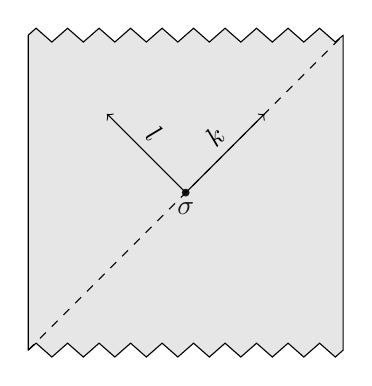
\begin{tikzpicture}
  \coordinate (tl) at (0, 4);
  \coordinate (tr) at (4, 4);
  \coordinate (bl) at (0, 0);
  \coordinate (br) at (4, 0);
  \coordinate (arrk) at (3, 3);
  \coordinate (arrl) at (1, 3);
  \coordinate[label=below:$\sigma$] (sig) at (2,2);

  
  \node at (sig) [circle, fill, inner sep=1pt]{};

  \begin{scope}[decoration={zigzag, segment length=0.4cm}]
    \draw[fill=gray, fill opacity=0.2] (tl) decorate {-- (tr)} to (br) decorate {-- (bl)} to (tl);
  \end{scope}

  \draw[dashed] (bl) to (tr);

  \draw[->] (sig) to node[midway, above left, sloped, pos=0.7] {$k$} (arrk);
  \draw[->] (sig) to node[midway, above right, sloped, pos=0.7] {$l$} (arrl);




\end{tikzpicture}
